\chapter{Linear Algebra and Calculus}
\section{Schur complement}
\begin{mytheorem}[Schur's complement]    
    Let 
    \begin{align}
        \mbf{A} &= 
        \bbm
            \mbf{A}_{11} & \mbf{A}_{12}\\
            \mbf{A}_{12} & \mbf{A}_{22}
        \ebm
    \end{align}
    be a square matrix. If $\mbf{A}_{11}$ is nonsingular, then the Schur complement of the block $\mbf{A}_{11}$ of the matrix $\mbf{A}$ is the matrix
    \begin{align}
        \mbf{A}/\mbf{A}_{11} := \mbf{A}_{22} - \mbf{A}_{21}\mbf{A}_{11}\inv\mbf{A}_{12}.
    \end{align}
    
    Similarly, if $\mbf{A}_{22}$ is nonsingular, then the Schur complement of the block $\mbf{A}_{22}$ of the matrix $\mbf{A}$ is the matrix
    \begin{align}
        \mbf{A}/\mbf{A}_{22} := \mbf{A}_{11} - \mbf{A}_{12}\mbf{A}_{22}\inv\mbf{A}_{21}.
    \end{align}
    \triqed
\end{mytheorem}

% \subsection{Application to solving linear equations}
% Given a system of equations 
% \begin{align}
%     \label{eq:schur solving lin system application}
%     \bbm
%             \mbf{A}_{11} & \mbf{A}_{12}\\
%             \mbf{A}_{21} & \mbf{A}_{22}
%     \ebm
%     \bbm \mbf{x}_{1}\\\mbf{x}_{2} \ebm 
%     &=
%     \bbm \mbf{b}_{1} \\\mbf{b}_{2} \ebm.
% \end{align}
% Then what is the solution $\mbf{x}_{1}$ without computing $\mbf{x}_{2}$ (or without solving the big system of equations all at once)?

% The solution is given by using the Schur complement of the block $\mbf{A}_{22}$ of the matrix $\mbf{A}$. Specifically, pre-multiply the left and right sides of \eqref{eq:schur solving lin system application} by the matrix
% \begin{align}
%     \mbf{L} &= 
%     \bbm
%         \eye & -\mbf{A}_{12}\mbf{A}_{22}\inv\\
%         \mbf{0} & \eye
%     \ebm.    
% \end{align}
% Then, the result is
% \begin{align}
%     \bbm
%         \eye & -\mbf{A}_{12}\mbf{A}_{22}\inv\\
%         \mbf{0} & \eye
%     \ebm
%     \bbm
%     \mbf{A}_{11} & \mbf{A}_{12}\\
%     \mbf{A}_{21} & \mbf{A}_{22}
%     \ebm
%     \bbm \mbf{x}_{1}\\\mbf{x}_{2} \ebm 
%     &=
%     \bbm
%         \eye & -\mbf{A}_{12}\mbf{A}_{22}\inv\\
%         \mbf{0} & \eye
%     \ebm
%     \bbm \mbf{b}_{1} \\\mbf{b}_{2} \ebm\\
%     %
%     \bbm
%         \mbf{A}_{11}-\mbf{A}_{12}\mbf{A}_{22}\inv\mbf{A}_{21} & \mbf{0}\\
%         \mbf{A}_{21} & \mbf{A}_{22}
%     \ebm
%     \bbm
%         \mbf{x}_{1}\\\mbf{x}_{2}
%     \ebm
%     &=
%     \bbm
%         \mbf{b}_{1} - \mbf{A}_{12}\mbf{A}_{22}\inv\mbf{b}_{2}\\
%         \mbf{b}_{2}
%     \ebm.
% \end{align}
% The solution $\mbf{x}_{1}$ is then given by solving
% \begin{align}
%     \left( \mbf{A}_{11}-\mbf{A}_{12}\mbf{A}_{22}\inv\mbf{A}_{21} \right)\mbf{x}_{1} 
%     &=
%     \mbf{b}_{1} - \mbf{A}_{12}\mbf{A}_{22}\inv\mbf{b}_{2}.
% \end{align}


% \subsection{Application in probability}
\subsection{Conditioning using covariance matrix}
Given a the random variable 
\begin{align}
    \bbm \mbfrv{x}_{1}\\\mbfrv{x}_{2} \ebm\sim\mc{N}\left( 
    \bbm \mbfbar{x}_{1}\\\mbfbar{x}_{2} \ebm,
    \bbm
    \mbs{\Sigma}_{11} & \mbs{\Sigma}_{12}\\
    \mbs{\Sigma}_{12}^{\trans} & \mbs{\Sigma}_{22}
    \ebm
    \right).
\end{align}
Then, the marginal covariance of $\mbfrv{x}_{1}$ is $\mbs{\Sigma}_{11}$. However, the covariance of $\mbfrv{x}_{1}$ \emph{given} $\mbfrv{x}_{2}=\mbfhat{x}_{2}$ is given by the Schur complement. Specifically,
\begin{align}
    \label{eq:condition covariance schur complement}
    \expect{\mbfrv{x}_{1}\middle|\mbfrv{x}_{2}=\mbfhat{x}_{2}} 
    &= \mbfbar{x}_{1} + \mbs{\Sigma}_{12}\mbs{\Sigma}_{22}\inv\left( \mbfhat{x}_{2}-\mbfbar{x}_{2} \right), \\
    \cov{\mbfrv{x}_{1}\middle|\mbfrv{x}_{2}=\mbfhat{x}_{2}} 
    &= \mbs{\Sigma}/\mbs{\Sigma}_{22}\\
    &= \mbs{\Sigma}_{11} - \mbs{\Sigma}_{12}\mbs{\Sigma}_{22}\inv\mbs{\Sigma}_{12}^{\trans}.
\end{align}

Note that this is equivalent to solving the linear system of equations
\begin{align}
    \label{eq:condition covariance linear system}
    \bbm
    \mbs{\Sigma}_{11} & \mbs{\Sigma}_{12}\\
    \mbs{\Sigma}_{12}^{\trans} & \mbs{\Sigma}_{22}
    \ebm
    \bbm \expect{\mbfrv{x}_{1}\middle|\mbfrv{x}_{2}=\mbfhat{x}_{2}} \\ \mbf{x}_{2}\ebm
    &=
    \bbm
    \mbfbar{x}_{1}\\
    \mbfbar{x}_{2} - \mbfhat{x}_{2}
    \ebm.
\end{align}
I'm not sure what's the relation between \eqref{eq:condition covariance linear system} and \eqref{eq:condition covariance schur complement}.
    
\subsection{Conditioning using information matrix}
On the other hand, if we are given the same random variable 
\begin{align}
    \bbm \mbfrv{x}_{1}\\\mbfrv{x}_{2} \ebm\sim\mc{N}\left( 
    \bbm \mbfbar{x}_{1}\\\mbfbar{x}_{2} \ebm,
    \bbm
        \mbf{A}_{11} & \mbf{A}_{12}\\
        \mbf{A}_{12}^{\trans} & \mbf{A}_{22}
    \ebm\inv
    \right),
\end{align}
where 
\begin{align}
    \mbf{A} = \mbs{\Sigma}\inv
\end{align}
is the \emph{information matrix}. Then, conditioning is easily done by partitioning the system. That is,
\begin{align}
    \cov{\mbfrv{x}_{1}\middle|\mbfrv{x}_{2}=\mbfhat{x}_{2}} 
    &= \mbf{A}_{11}\inv.
\end{align}
On the other hand, marginalization is more ``difficult'' and is given by the Schur complement. Specifically,
\begin{align}
    \cov{\mbfrv{x}_{1}} &= \left( \mbf{A}/\mbf{A}_{22} \right)\inv\\
    &= \left( \mbf{A}_{11}-\mbf{A}_{12}\mbf{A}_{22}\inv\mbf{A}_{12}^{\trans} \right)\inv.
\end{align}

\section{Liebniz rule for integration}
\begin{definition}[Liebniz rule]
    \begin{align}
        \f{\dee}{\dee x}\left(\int_{a(x)}^{b(x)} f(x, t) \dee t\right)=f(x, b(x)) \cdot \frac{\dee}{\dee x} b(x)-f(x, a(x)) \cdot \frac{\dee}{\dee x} a(x)+\int_{a(x)}^{b(x)} \pd{}{x} f(x, t) \dee t.
    \end{align}
\end{definition}


\chapter{Numerically sampling from a normal distribution}
Say we want to sample realizations of a normal random variable $\mbfrv{x}\sim\mc{N}(\mbs{\mu}_{x},\mbs{\Sigma})$, given the mean $\mbs{\mu}_{x}$ and covariance $\mbs{\Sigma}_{x}$. How can this be done using MATLAB's \texttt{randn} function?

\section{MATLAB's \texttt{randn} function}
The \texttt{randn} function produces a realization of a normal random variable with zero mean and unit variance. How to compute the variance of such variable? Well, that depends on how the realizations are stored in MATLAB. That is, the realizations can be stored as columns or as rows. 

Say the random variable has $n$ degrees of freedom and we want $m$ realizations. Thus, if the realizations are stored as columns, then the matrix is of size $n\times m$. On the other hand, if the realizations are stored as rows, then the matrix of size $m\times n$. Specifically,
\begin{align}
    \mbf{x}_{\mathrm{unit, col}} &= \texttt{randn(n,m)}\in\rnums^{n\times m},\\
    \mbf{x}_{\mathrm{unit, row}} &= \texttt{randn(m,n)}\in\rnums^{m\times n}.
\end{align}
The covariance of $\mbf{x}_{\mathrm{unit}}$ can be approximated numerically as
\begin{align}
    \cov{\mbf{x}_{\mathrm{unit}}} 
    &= \mbs{\Sigma}_{\mathrm{unit}}\\
    &= \eye_{n\times n}\\
    \label{eq:unit covariance col. realizations}
    &\approx \f{1}{m-1}\mbf{x}_{\mathrm{unit, col}}\mbf{x}_{\mathrm{unit, col}}^{\trans}\\
    \label{eq:unit covariance row. realizations}
    &= \f{1}{m-1}\mbf{x}_{\mathrm{row, unit}}^{\trans}\mbf{x}_{\mathrm{row, unit}}.
\end{align}

Well, what if we want a realization of a normal random variable with zero mean but non-unit variance $\mbs{\Sigma}_{x}$? The covariance is then
\begin{align}
    \cov{\mbf{x}} 
    &= \mbs{\Sigma}_{x}\\
    &= \mbf{L}\underbrace{\mbs{\Sigma}_{\mathrm{unit}}}_{\eye}\mbf{L}^{\trans}\\
    &= \mbf{R}^{\trans}\underbrace{\mbs{\Sigma}_{\mathrm{unit}}}_{\eye}\mbf{R},
\end{align}
where $\mbf{L}$ and $\mbf{R}$ are the lower- and upper-triangular matrices obtained from the Cholesky factorization. So which of these two should we use? Well, the answer depends on how the realizations of $\mbfrv{x}$ are stored. 


If the realizations are stored in columns, then from \eqref{eq:unit covariance col. realizations}, 
\begin{align}
    \cov{\mbf{x}}
    &= \mbs{\Sigma}_{x}\\
    &=  \mbf{L}\mbs{\Sigma}_{\mathrm{unit}}\mbf{L}^{\trans}\\
    &\approx \mbf{L}\mbf{x}_{\mathrm{unit,col}}\mbf{x}_{\mathrm{unit,col}}^{\trans}\mbf{L}^{\trans}\\
    &= \underbrace{\left(\mbf{L}\mbf{x}_{\mathrm{unit,col}}\right)}_{\mbf{x}_{\mathrm{col}}}\left(\mbf{L}\mbf{x}_{\mathrm{unit, col}}\right)^{\trans}\\
    &= \mbf{x}_{\mathrm{col}}\mbf{x}_{\mathrm{col}}^{\trans},
\end{align}
where
\begin{align}
    \mbf{x}_{\mathrm{col}} &= \mbf{L}\mbf{x}_{\mathrm{unit, col}}\\
    &= \mbf{L}\texttt{randn(n,m)}.
\end{align}
It should be noted that if $\mbf{R}$ is used in place of $\mbf{L}$, then the results would not be the same in general. The upper triangular matrix $\mbf{R}$ can still be used by setting
\begin{align}
    \mbf{L} &= \mbf{R}^{\trans}.
\end{align}
Specifically,
\begin{align}
    \cov{\mbf{x}}
    &= \mbs{\Sigma}_{x}\\
    &=  \mbf{R}^{\trans}\mbs{\Sigma}_{\mathrm{unit}}\mbf{R}\\
    &\approx \mbf{R}^{\trans}\mbf{x}_{\mathrm{unit,row}}^{\trans}\mbf{x}_{\mathrm{unit,row}}\mbf{R}\\
    &= \left(\mbf{x}_{\mathrm{unit, row}}\mbf{R}\right)^{\trans}\underbrace{\left(\mbf{x}_{\mathrm{unit,row}}\mbf{R}\right)}_{\mbf{x}_{\mathrm{row}}}\\
    &= \mbf{x}_{\mathrm{row}}^{\trans}\mbf{x}_{\mathrm{row}},
\end{align}
where
\begin{align}
    \mbf{x}_{\mathrm{row}} &= \mbf{x}_{\mathrm{unit, row}}\mbf{R}\\
    &= \texttt{randn(m,n)}\mbf{R}.
\end{align}


\begin{myBlueBox}
    \textbf{Summary}: 
    \begin{align}
        \mbs{\Sigma}_{x} &= \mbf{R}^{\trans}\mbf{R}\\
        &= \mbf{L}\mbf{L}^{\trans},\\
        \mbf{x}_{\mathrm{unit, col}} &= \texttt{randn(n,m)}\\
        &= \mbf{x}_{\mathrm{unit, row}}^{\trans},\\
        \mbf{x}_{\mathrm{col}} &= \mbf{L}\mbf{x}_{\mathrm{unit, col}},\\
        &= \mbf{x}_{\mathrm{row}}^{\trans},\\
        \mbf{x}_{\mathrm{row}}&= \mbf{x}_{\mathrm{unit, row}}\mbf{R}.
    \end{align}
\end{myBlueBox}

%%%%%%%%%%%%%%%%%%%%%%%%%%%%%%%%%%%%%%%%%%%%%%%%%%%%%%%%%%%%
%%%%%%%%%%%%%%%%%%%%%%%%%%%%%%%%%%%%%%%%%%%%%%%%%%%%%%%%%%%%
\section{Sampling (another derivation)}
Assume we have $N$ realizations $\mbf{x}\in\rnums^{n\times N}$ of the random variable $\mbfrv{x}\in\rnums^{n}$. For simplicity, we'll assume the random variable has zero mean. 
% Then the covariance matrix can be estimated as 
% \begin{align}
%     {\mbs{\Sigma}} \approx \f{1}{N-1}\sum_{i=1}^{N} \mbf{x}_{i}\mbf{x}_{i}^{\trans}.
% \end{align}
% 
Let's assume that there exists a matrix $\mbf{R}$ such that
\begin{align}
    \mbfrv{x} &= \mbf{R}\mbfrv{x}_{0},
\end{align}
where $\mbfrv{x}_{0}\sim{N}\left( \mbf{0},\eye \right)$. Then,
\begin{align}
    \mbs{\Sigma} &= \expect{\mbfrv{x}\mbfrv{x}^{\trans}}\\
     &= \mbf{R}\expect{\mbfrv{x}_{0}\mbfrv{x}_{0}^{\trans}}\mbf{R}^{\trans}\\
     &= \mbf{R}\mbf{R}^{\trans}.
\end{align}
well, how can we construct $\mbf{R}$? Decompose the covariance matrix using eigendecomposition. Specifically,
\begin{align}
    \mbs{\Sigma} 
    &= \mbf{U}\mbs{\Lambda}\mbf{U}^{\trans}\\
    &= \underbrace{\mbf{U}\sqrt{\mbs{\Lambda}}}_{\mbf{R}}\eye\underbrace{\sqrt{\mbs{\Lambda}}\mbf{U}^{\trans}}_{\mbf{R}^{\trans}}\\
    &= \mbf{R}\mbf{R}^{\trans},
\end{align}
where $\mbf{U}$ and $\mbs{\Lambda}$ are the eigenvector and the eigenvalue matrices, respectively. 
Thus, 
\begin{align}
    \mbf{R} &= \mbf{U}\sqrt{\mbs{\Lambda}}.
\end{align}
Therefore, the random variable $\mbfrv{x}$ can be sampled by sampling from the unit normal random variable $\mbfrv{x}_{0}$ and scaling it using
\begin{align}
    \mbf{x} &= \mbf{U}\sqrt{\mbs{\Lambda}}\mbf{x}_{0}.
\end{align}

%%%%%%%%%%%%%%%%%%%%%%%%%%%%%%%%%%%%%%%%%%%%%%%%%%%%%%%%%%%%
%%%%%%%%%%%%%%%%%%%%%%%%%%%%%%%%%%%%%%%%%%%%%%%%%%%%%%%%%%%%

\section{Covariance ellipses}
To plot covariance ellipses (in 2D), eigendecomposition is used. Specifically, given a covariance matrix $\mbs{\Sigma}$, then decompose 
\begin{align}
    \mbs{\Sigma} &= \mbf{U}\mbs{\Lambda}\mbf{U}^{\trans},
\end{align}
where $\mbf{U}\inv=\mbf{U}^{\trans}$ because $\mbs{\Sigma}=\mbs{\Sigma}^{\trans}$ is symmetric. The standard deviation ellipses\footnote{I'm not sure about the naming here. But the ellipse computed represents the 1$\sigma$ bounds.} are the computed as
\begin{align}
    \mbs{\sigma} &= \mbf{U}\sqrt{\mbs{\Lambda}}\bbm \cos(\theta)\\\sin(\theta) \ebm, \qquad \theta\in[0,2\pi).
\end{align}
Figure~\ref{fig:Example covariance ellipses} shows an example of such ellipses. 
\begin{figure}[h]
    \centering
    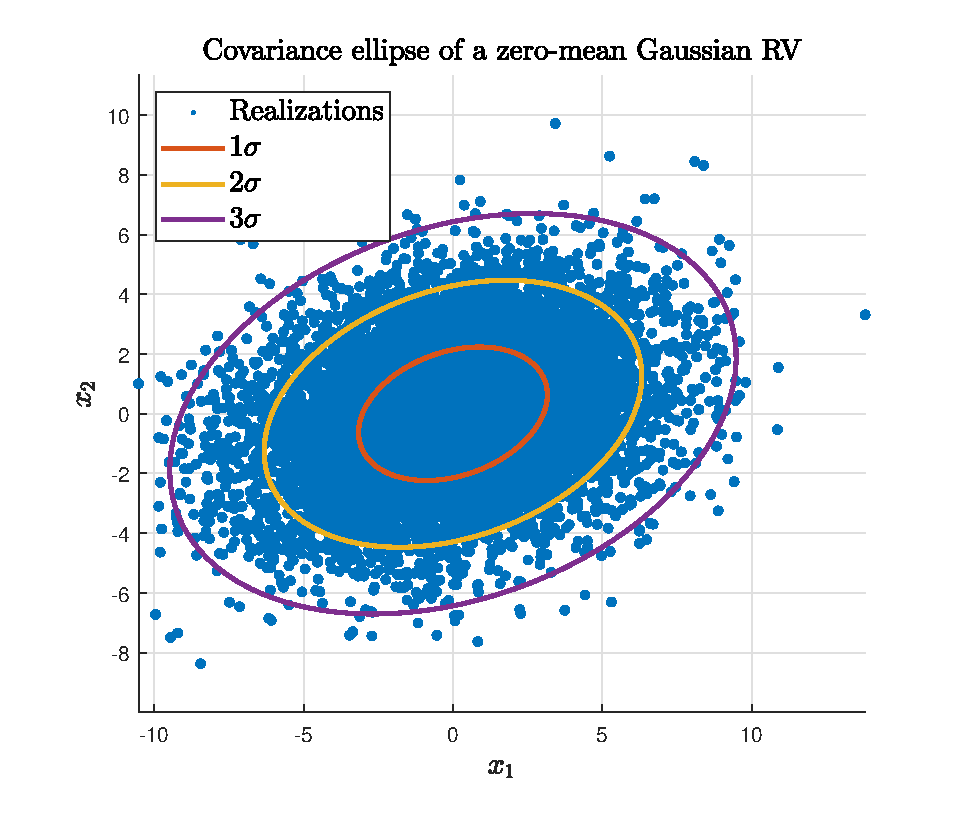
\includegraphics[width=0.8\textwidth]{figs/Covariance_ellipses_example.eps}    
    \caption{Covariance ellipses (actually, standard deviation ellipses) around $N=10^{4}$ samples.}
    \label{fig:Example covariance ellipses}
\end{figure}


%%%%%%%%%%%%%%%%%%%%%%%%%%%%%%%%%%%%%%%%%%%%%%%%%%%%%%%%%%%%
%%%%%%%%%%%%%%%%%%%%%%%%%%%%%%%%%%%%%%%%%%%%%%%%%%%%%%%%%%%%
\section{Generating positive definite matrices}
Symmetric positive definite (SPD) matrices are a subset of Matrix Lie Groups \cite{arsigny_geometric_2007}. The Lie algebra is the set of all symmetric matrices. Thus, taking the exponential map of a symmetric matrix gives a symmetric positive definite matrix \cite[Prop.~3.4]{arsigny_geometric_2007}.
\begin{proposition}[Exponential map of symmatric matrices]
    From \cite[Prop.~3.4]{arsigny_geometric_2007}. Let $\mbf{S}\in \mathrm{Sym}(n)$ be a symmetric matrix. Then,
    \begin{align}
        \exp\left( \mbf{S} \right) \in \mathrm{Sym}^{+}_{\star}(n),
    \end{align}
    where $\mathrm{Sym}^{+}_{\star}$ is the set of symmetric positive definite matrices. 
\end{proposition}
